\documentclass{article}

% The paper: MicroInfer and semantic-aware adaptive KV cache precision, in the
% NeurIPS 2026 format (docs/neurips_2026.sty, from the official formatting
% instructions). Every figure quoted must come from
% experiments/logs/benchmark.jsonl; entries are cited by their sha256 prefix in
% the ADRs. The main text must stay within nine pages.

% Numeric citations, so that \cite reads as [n].
\PassOptionsToPackage{numbers, compress}{natbib}

% Submission: anonymised, with line numbers. Add "preprint" for arXiv, or
% "final" once accepted.
\usepackage{neurips_2026}

\usepackage[utf8]{inputenc}
\usepackage[T1]{fontenc}
\usepackage{hyperref}
\usepackage{url}
\usepackage{booktabs}
\usepackage{amsmath}
\usepackage{amsfonts}
\usepackage{nicefrac}
\usepackage{microtype}
\usepackage{xcolor}
\usepackage{tikz}
\usetikzlibrary{positioning, arrows.meta}

\title{Keeping Local LLM Inference Alive under Video Memory Contention by
Reallocating KV Cache Precision at Runtime}

% Hidden in the anonymised submission; filled in for the final version.
\author{%
  Anonymous Author(s) \\
  Affiliation \\
  Address \\
  \texttt{email} \\
}

\begin{document}

\maketitle

\begin{abstract}
Large language models increasingly run on personal hardware, where the graphics
processor is shared with a browser, a video player and an editor, and offers no
memory isolation between them. When another process takes video memory, a
generation session that fitted a moment earlier ends with an out-of-memory
error and loses its context. Adaptive serving systems assume a datacenter, with
a dedicated accelerator and a scheduler that sees the workload; key-value cache
quantisation, uniform or mixed-precision, fixes its compression budget before
the session begins. We present \textit{MicroInfer}, an inference engine built
from scratch in which every page of the key-value cache carries its own
precision tier among FP16, INT8, INT4 and INT2. A monitor polls the driver and
classifies free memory into three pressure levels with thresholds derived from
measured contention; an importance scorer accumulates each page's attention
mass inside the attention kernel; and a controller meets a byte target by
downgrading the pages whose loss costs least per byte, restoring them exactly
from a full-precision copy in host memory once pressure passes. Freed memory is
returned to the driver through the virtual memory management interface, so the
saving is visible to the other process and to the measurement. On a 6\,GiB
laptop GPU, everyday applications take hundreds of MiB and mostly keep them;
the monitor detects every catchable episode within 246\,ms with no false
alarm; and with Qwen2.5-1.5B at 32K positions, a contention that runs the
static engine out of memory is survived by the adaptive one, which returns
746\,MiB that the driver sees returned, to a granule, at every plan.
\end{abstract}

% =====================================================================
\section{Introduction}
\label{sec:introduction}

Large language models are increasingly run on personal hardware. Openly
released models of one to a few billion parameters \cite{qwen2024report},
together with tools such as Ollama \cite{ollama} and llama.cpp \cite{llamacpp},
make it ordinary to hold a conversation with a model on a laptop, for privacy,
offline use, and the absence of a per-token bill. Wherever a model runs, its
inference is bound by memory: generating a token reads every weight and every
cached key and value, and in datacenter serving the memory the key-value cache
takes is what limits how many requests are served at once
\cite{kwon2023pagedattention}. On a laptop the limit is tighter, a few GiB of
video memory for weights, cache and working space together.

On a consumer graphics processor that memory is not even fixed. Unlike a
datacenter accelerator partitioned by MIG or MPS, a consumer GPU offers no
memory isolation between the processes that share it: video memory goes to
whoever asks first, and no process is told when another takes more. A session
that fits comfortably can then fail outright when a browser tab starts playing
video. The failure is not degradation but termination: the session ends and its
cached context is lost. On the 6\,GiB laptop GPU used here, everyday
applications take hundreds of MiB and mostly keep them, which brings a long
session to within a few hundred MiB of that failure (Section~\ref{sec:rq1}).

What makes the problem tractable is that a model's footprint is not
monolithic. Its weights are fixed for a session, but its key-value cache grows
with every token and can be held at varying precision; at a long context,
compressing it frees as much memory as an everyday application takes. We ask
whether that trade can be made \textit{during} a session, in response to
pressure the engine did not cause, and whether the loss can be concentrated on
the cached positions the model attends to least.

Existing work holds parts of the answer (Section~\ref{sec:related}). Adaptive
serving systems change memory allocation at runtime, but for pressure that
comes from the requests they admit. Consumer engines run in the right place,
but fix capacity when the model loads. Uniform cache quantisation settles how
far a cache can be compressed, and mixed-precision quantisation shows that
precision is better spent unevenly, guided by attention or sensitivity; both
fix their budget before the session. Attention-guided eviction has the right
signal but discards irreversibly. No system reallocates cache precision at
runtime, non-uniformly, in response to memory taken by processes it cannot see,
and restores it afterwards.

This paper asks three questions, each answered by a component of the system.
\textbf{RQ1:} how volatile is free video memory on a consumer laptop under
everyday use? We record it at 50\,Hz while a script plays everyday
applications, and analyse every spike by a rule fixed before recording.
\textbf{RQ2:} can a runtime that consults no scheduler detect pressure, and
survive it? A monitor polls the driver with thresholds set by a rule from RQ1's
spikes, and a controller downgrades cache pages to meet a byte target; we score
the monitor against an independent ground truth and run a session through
contention that ends the static engine. \textbf{RQ3:} does allocating
precision by attention preserve task quality better than allocating it
uniformly, at equal compression? Three score sources plug into the same
planner, so that they reclaim the same bytes and differ only in which pages they
degrade.

Our contributions are:
\begin{itemize}
\item \textbf{A characterisation of video memory contention on a consumer
laptop}, attributed to the processes that cause it: spikes are large (P90
506\,MiB), rise over seconds (median 1.09\,s) and mostly persist (45 of 48).
\item \textbf{A scheduler-agnostic pressure monitor} whose thresholds follow
from that measurement by a fixed rule, and which detected all 84 catchable RED
episodes within 246\,ms with no false alarm.
\item \textbf{A runtime precision policy and the engine that runs it}: a paged
cache whose pages change tier between decoding steps, every move quantising
from an FP16 shadow so that upgrades restore exactly, freed memory returned to
the driver, and a marginal-cost planner over attention-derived importance. It
survives, at 32K positions, a contention that ends the static engine.
\item \textbf{An evaluation design that isolates allocation from compression},
holding the reclaimed bytes equal between semantic, uniform and random
allocation.
\end{itemize}

% =====================================================================
\section{Background and related work}
\label{sec:related}

\paragraph{The key-value cache.} Decoding attends over all previous positions
\cite{vaswani2017attention}, so their keys and values are cached. The cache
takes $2 \cdot L \cdot h_{kv} \cdot d_h \cdot n \cdot s$ bytes for $L$ layers,
$h_{kv}$ key-value heads of dimension $d_h$, $n$ positions and $s$ bytes per
element. Of these, only $n$ and $s$ change during a session, and $n$ is the
user's: bytes per element is the one term an engine can renegotiate. On
Qwen2.5-1.5B a position takes 28\,KiB at FP16, so 32K positions take 896\,MiB;
at a short context, compressing the whole cache frees less than a browser tab
takes, which fixes our experimental configuration at a long one.

\paragraph{Video memory on consumer GPUs.} Free memory is observable only by
polling the driver \cite{nvml}, and only memory returned to the driver is
visible there: a caching allocator that keeps freed memory makes it look like
contention. The CUDA virtual memory management interface \cite{cudavmm}
reserves address ranges independently of physical memory, so a cache can map
memory granule by granule and give it back.

The related work falls into five families, which we take from the furthest from
this work to the closest.

\paragraph{Adaptive serving.} PagedAttention \cite{kwon2023pagedattention}
manages the cache in blocks inside a reservation taken at start-up. FineServe
\cite{fineserve} serves models of heterogeneous precision, MorphServe
\cite{morphserve} swaps in quantised layers and resizes the cache with the
workload, Oneiros \cite{mirage} remaps parameter memory to hold more cache, and
eLLM \cite{ellm} manages memory elastically. They show runtime adaptation is
worthwhile, but assume a dedicated accelerator, a scheduler that sees the
pressure coming, and many requests to trade between; and memory kept in a
private reservation is never returned to the driver.

\paragraph{Consumer and edge inference.} llama.cpp \cite{llamacpp} and Ollama
\cite{ollama} bring quantised models to personal machines, PowerInfer
\cite{song2024powerinfer} splits work between GPU and CPU by neuron activity,
and FlexGen \cite{sheng2023flexgen} offloads to host memory and disk. They
treat capacity as fixed when the model loads.

\paragraph{Uniform cache quantisation.} KVQuant \cite{hooper2024kvquant} and
KIVI \cite{liu2024kivi} show that the cache tolerates aggressive quantisation;
KIVI quantises keys per channel and values per token and reaches two bits. We
adopt KIVI's quantiser. Its precision is chosen once, before the session, and
identically for every position.

\paragraph{Attention-guided eviction.} H2O \cite{zhang2023h2o} keeps the tokens
that accumulate attention, StreamingLLM \cite{xiao2024streamingllm} keeps the
initial ``attention sink'' with a recent window, and Ada-KV
\cite{feng2024adakv} spreads the budget across heads. We borrow the signal;
eviction itself is irreversible and its budget fixed.

\paragraph{Mixed-precision cache quantisation.} The closest family varies
precision across the cache: KVTuner \cite{kvtuner} by layer from offline
sensitivity, MiKV \cite{yang2024mikv} by keeping tokens an eviction policy would
drop at low precision, ZipCache \cite{he2024zipcache} by salient tokens found
from normalised attention, and Cocktail \cite{tao2025cocktail} by chunk from
similarity to the query. They distribute a budget fixed in advance and observe
nothing of the memory the device has left, and none raises precision again.

% =====================================================================
\section{Design}
\label{sec:design}

\subsection{Overview}
\label{sec:overview}

\textit{MicroInfer} has two layers (Figure~\ref{fig:overview}). The
\textbf{engine} runs the model over CUDA kernels written for this work and
holds the cache on \textit{pages}, the keys and values of $P = 32$ consecutive
positions of one layer, each at a \textit{tier}: FP16, INT8, INT4 or INT2. The
\textbf{control loop} decides which page is held at which tier: a pressure
monitor, an importance scorer, a precision controller, and the cache manager
that applies its plans. Plans are applied between decoding steps, never inside
a kernel launch, so no kernel sees the cache half converted.

\begin{figure}[t]
\centering
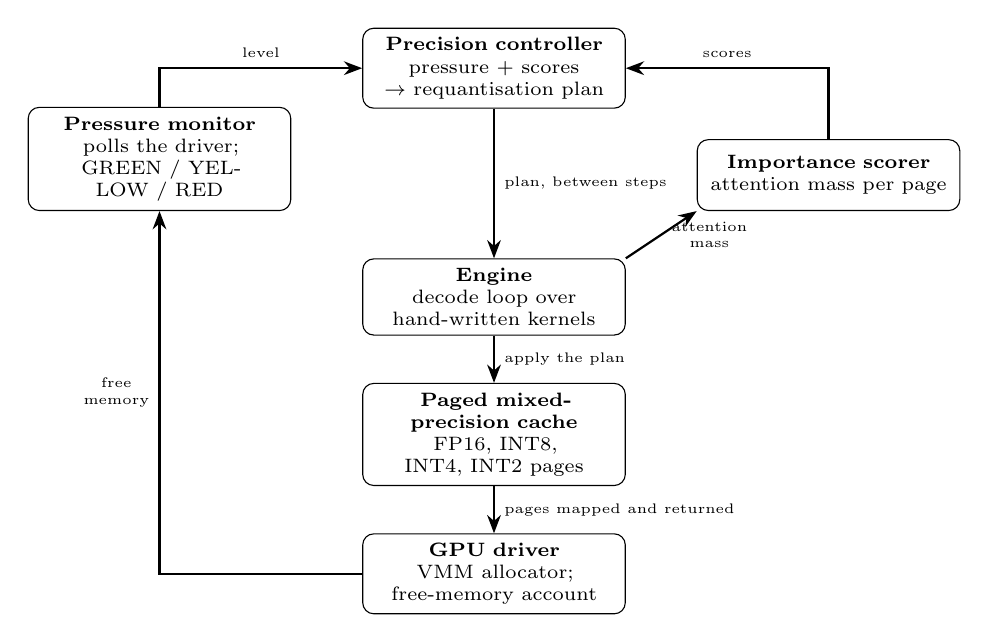
\begin{tikzpicture}[
  box/.style={draw, rounded corners, align=center, minimum height=0.9cm,
              text width=3.1cm, font=\scriptsize},
  arrow/.style={-{Stealth}, thick},
  note/.style={font=\tiny, align=center},
  node distance=0.6cm and 0.9cm]
  \node[box] (engine) {\textbf{Engine}\\decode loop over\\hand-written kernels};
  \node[box, above left=of engine] (monitor) {\textbf{Pressure monitor}\\polls the driver;\\GREEN / YELLOW / RED};
  \node[box, above right=of engine] (scorer) {\textbf{Importance scorer}\\attention mass per page};
  \node[box, above=1.9cm of engine] (controller) {\textbf{Precision controller}\\pressure + scores\\$\rightarrow$ requantisation plan};
  \node[box, below=of engine] (cache) {\textbf{Paged mixed-precision cache}\\FP16, INT8, INT4, INT2 pages};
  \node[box, below=of cache] (driver) {\textbf{GPU driver}\\VMM allocator;\\free-memory account};
  \draw[arrow] (driver.west) -| node[note, pos=0.75, left] {free\\memory} (monitor.south);
  \draw[arrow] (monitor.north) |- node[note, pos=0.75, above] {level} (controller.west);
  \draw[arrow] (engine.north east) -- node[note, right] {attention\\mass} (scorer.south west);
  \draw[arrow] (scorer.north) |- node[note, pos=0.75, above] {scores} (controller.east);
  \draw[arrow] (controller.south) -- node[note, right] {plan, between steps} (engine.north);
  \draw[arrow] (engine.south) -- node[note, right] {apply the plan} (cache.north);
  \draw[arrow] (cache.south) -- node[note, right] {pages mapped and returned} (driver.north);
\end{tikzpicture}
\caption{\textit{MicroInfer}: the engine, and the control loop that decides the
precision tier of each page of its key-value cache. Freed memory returns to the
driver, where the monitor and other processes see it.}
\label{fig:overview}
\end{figure}

\subsection{The pressure monitor}
\label{sec:monitor}

A background thread polls the driver's free memory, the \textit{headroom},
every 50\,ms on absolute deadlines. Headroom below $T_\mathrm{low}$ is RED,
below $T_\mathrm{high}$ YELLOW, else GREEN; thresholds are absolute, since
contention is. A new level is reported once $K$ consecutive polls agree, so a
drop shorter than $K$ polls is never reported and a clean change is reported
within $K+1$. Each transition is queued as an event, with the memory held by
the engine and by every other process.

The thresholds follow from RQ1 by a fixed rule, not by tuning. RED is headroom
below a spike at the P90 amplitude, rounded up to 64\,MiB; $K$ is the largest
number of polls whose detection time, $(K+1) \times 50$\,ms, does not exceed the
P10 rise time; YELLOW adds what a fast spike takes while it is detected and a
plan applied. RQ1's spikes give RED below 512\,MiB, $K = 3$ and YELLOW below
1024\,MiB.

\subsection{The mixed-tier paged cache}
\label{sec:cache}

Quantised tiers follow KIVI \cite{liu2024kivi}: keys asymmetric with a scale
and zero-point per (head, channel) across the page, values per (head,
position). One layout serves every tier; its 1280 bytes of metadata per page
on Qwen2.5-1.5B make INT8, INT4 and INT2 cost 8.63, 4.63 and 2.63 effective
bits per element, and every compression ratio here counts it. A page being
filled stays at FP16, since a key channel's scale spans the whole page.

Each tier has its own virtual address range, reserved through the VMM interface
for the whole context window. Physical memory is mapped a 2\,MiB granule at a
time as pages arrive; a tier's live pages occupy its lowest slots, freeing a
page moves the tier's last page into its slot, and an empty granule is returned
to the driver. One attention kernel reads every page at the tier the page table
records for it, dequantising as it loads, in a single pass; query tiles are
aligned to pages, so a tile reads one tier.

\subsection{Runtime requantisation}
\label{sec:requantisation}

A downgrade allocates the page at the target tier while the old page is still
read, quantises it, points the page table at it, and frees the old page; if
the allocation fails, nothing has changed. Before a page's first downgrade its
FP16 bytes are copied to pinned host memory, its \textit{shadow}, and every
move quantises from FP16, never from the current codes. A page at tier $T$ is
therefore always exactly the quantisation of its rows at $T$: each tier has one
error, and errors do not compound along a page's path. An upgrade copies or
quantises from the shadow; to FP16 it restores the page bit for bit. Decoding
the codes back up was rejected, since it would give FP16's size at the lower
tier's error. A move of one page of one layer takes 8 to 39\,$\mu$s at the
median on Qwen2.5-1.5B (Appendix~\ref{app:moves}), and the shadows of a whole
32K cache take about 0.9\,GiB of host memory.

\subsection{The importance scorer}
\label{sec:scorer}

The attention kernel computes the softmax online, one page per tile. On
request each tile writes its partial $\sum \exp(s - m)$ with its maximum $m$,
and once the softmax's final maximum and sum are known these are normalised
into each page's share of the attention mass, with no second pass over the
cache. Averaged over a layer's query heads, the mass $\bar a_{\ell,i}$ of page
$i$ in layer $\ell$ is folded on the device into
$\mathrm{score}_{\ell,i} \leftarrow \alpha\,\bar a_{\ell,i} + (1-\alpha)\,
\mathrm{score}_{\ell,i}$ with $\alpha = 0.2$, a page's first observation
seeding its score. Folding every step cost Qwen2.5-0.5B 0.71\% of decode
throughput, outside noise; every fourth step is within noise on both models and
is the default. Attention sinks get no special protection: unaided, the scorer
rates the first page highest when averaged over layers.

\subsection{The precision controller}
\label{sec:controller}

The controller, pure logic with no device code, turns the level, the headroom,
the scores and the tiers into a plan. It reclaims what brings headroom back
above YELLOW with a 64\,MiB margin, $T_\mathrm{high} + 64\,\mathrm{MiB} -
\text{headroom}$, rather than a fixed fraction of the cache. It meets this
target greedily, repeatedly taking the cheapest next move of one page one tier
down by marginal cost
\begin{equation}
  c_{\ell,i}(t \to t') = \mathrm{score}_{\ell,i}\,
    \frac{e(t') - e(t)}{b(t) - b(t')},
  \label{eq:marginal}
\end{equation}
where $e$ is a tier's relative mean squared error from offline round trips and
$b$ its bytes per page. Equal scores give breadth first, since each tier down
costs more per byte than the last; a page the model hardly attends to goes deep
first. The open pages and the last 128 positions are never downgraded.
Upgrades come at GREEN only, largest gain first, at least 5\,s after the later
of the last downgrade and the end of pressure, and never below $T_\mathrm{high}
+ 512$\,MiB of headroom. Three \textit{score sources} plug into the same
planner and meet the same byte target to within one page's move: the scorer's
(\textit{semantic}), equal scores spread evenly across positions
(\textit{uniform}, the baseline), and seeded random scores.

\paragraph{The engine's reaction.} On YELLOW the engine applies the plan a
batch per step within 20\,ms; on RED, all at once; while the level persists it
plans again as the cache seals pages. If an allocation fails outright, an
emergency plan for no headroom is applied and the step retried once; failing
that, the generation ends gracefully with the tokens it produced. Because events
are drained only between steps, and a 512-position prefill chunk at 16K--24K
positions takes 11--16\,s, prefill chunks are sized under pressure from a model
of a step's cost, a fixed part plus a part per position, so that a step takes
about 0.8\,s, or about twice its fixed part where the fixed part alone exceeds
that. At GREEN chunks stay at 512 positions.

% =====================================================================
\section{Implementation}
\label{sec:implementation}

\textit{MicroInfer} is a Python orchestrator over CUDA kernels written for
this work: embedding, RMSNorm, rotary embeddings, SwiGLU, attention over
contiguous, paged and quantised pages, the paged cache and its VMM allocator,
quantisation at every tier, and greedy sampling. No inference engine is used.
The one exception is the dense projections, which call cuBLAS
\cite{cublas} with fp32 accumulation; hand-written GEMMs ran 8--28 times slower
at 512 rows, and would have confounded every latency we report with the cost of
a slow matrix multiplication (Appendix~\ref{app:boundary}). No deep learning
framework runs beside the engine, whose caching allocator would hide freed
memory from the driver. Every figure below is drawn from a hash-chained
benchmark log whose entries name the code that produced them.

% =====================================================================
\section{Evaluation}
\label{sec:evaluation}

All measurements are on one laptop with an NVIDIA RTX 4050 Laptop GPU (6\,GiB,
6141\,MiB reported by the driver), under Linux with a GNOME desktop whose
processes share the GPU throughout. The experimental configuration is
Qwen2.5-1.5B at 32K positions with its cache at FP16, which leaves about
1.2\,GB of headroom: the range in which realistic contention decides whether a
session survives.

\subsection{RQ1: contention on a consumer laptop}
\label{sec:rq1}

A script played everyday actions, labelling each in the trace: a browser with
1, 5 and 10 tabs, YouTube at 1080p and 2160p, a WebGL page, a 2160p video in
VLC, and VS Code. A recorder sampled free memory at 50\,Hz and each process's
memory at 5\,Hz. The scenario was recorded five times with the engine holding
32K positions and once without it, 2.2 hours in all, and analysed by a spike
definition fixed beforehand (Appendix~\ref{app:spikes}): free memory at least
64\,MiB below a rolling 5\,s median for at least 100\,ms.

\begin{table}[t]
\caption{Spikes at the 64\,MiB threshold in six recordings, by the action in
progress. Contention is large, and a video player takes the most.}
\label{tab:rq1}
\centering
\small
\begin{tabular}{lrrr}
\toprule
Action & Spikes & Median amplitude (MiB) & Largest (MiB) \\
\midrule
Browser, 10 tabs & 7 & 220 & 284 \\
Browser, 1 tab & 6 & 150 & 167 \\
VLC, 2160p video & 6 & 526 & 567 \\
YouTube, 1080p / 2160p & 5 / 5 & 101 / 181 & 292 / 196 \\
VS Code & 5 & 91 & 94 \\
Engine prefill & 5 & 182 & 182 \\
WebGL page & 4 & 100 & 138 \\
Other & 5 & 85--103 & 103 \\
\bottomrule
\end{tabular}
\end{table}

The six recordings hold 48 spikes (98 at 32\,MiB, 28 at 128\,MiB;
Table~\ref{tab:rq1}). \textbf{Contention mostly stays:} 45 of the 48 are lasting
drops, an application keeping its memory until it closed, so reclaiming memory
once is not enough. \textbf{It is large:} a median of 154\,MiB, a P90 of
506\,MiB, and at most 567\,MiB. \textbf{It rises over seconds:} a median of
1.09\,s from 10\% to 90\% of the amplitude, and a P10 of 242\,ms. Attribution
named a process for 44 spikes, mostly the browser's GPU process. Beside the
engine at 32K the lowest headroom was 377\,MiB: contention brings a long
session within a few hundred MiB of failure.

\subsection{RQ2: detecting pressure}
\label{sec:detection}

The monitor was scored against a truth it has no part in: the recorder's own
50\,Hz trace with the monitor's thresholds applied. A \textit{true RED episode}
is a run of samples below RED; its \textit{detection latency} runs to the first
RED event that reports it, and an episode of 100\,ms or more with none is a
false negative; a RED event with no true RED is a false positive. Episodes
shorter than $K+1$ polls and a sample, 220\,ms, are counted apart. While
Qwen2.5-1.5B held a generation, a contention simulator, a process of its own
taking memory through the engine's allocator (Appendix~\ref{app:simulator}),
played a grid of 36 pulse shapes three times each, or replayed RQ1's five
with-engine recordings.

\begin{table}[t]
\caption{The monitor against the recorder's truth: true RED episodes, those long
enough to catch, false negatives (FN), false negatives shorter than $K+1$
polls, false positives (FP), and detection latency. Every catchable episode was
caught, with no false alarm.}
\label{tab:detection}
\centering
\small
\begin{tabular}{lrrrrrr}
\toprule
Workload & RED & Catchable & FN & FN under $K$ & FP & Latency, median / max (ms) \\
\midrule
Synthetic grid & 67 & 57 & 0 & 2 & 0 & 126 / 246 \\
RQ1 replayed & 30 & 27 & 0 & 0 & 0 & 114 / 143 \\
\bottomrule
\end{tabular}
\end{table}

Over the 84 catchable episodes there were no false negatives and no false
positives (Table~\ref{tab:detection}). Detection took about two and a half
polls, at most 246\,ms, against a median spike rise of 1.09\,s. The two missed
episodes came from pulses with a sheer edge and a 0.1\,s plateau, shorter than
the three polls the monitor needs; RQ1's recordings held none that short. The
monitor costs decoding nothing measurable: $+0.17\%$ on Qwen2.5-0.5B and
$-0.32\%$ on Qwen2.5-1.5B, both within twice their standard error.

\subsection{RQ2: surviving pressure}
\label{sec:survival}

Qwen2.5-1.5B prefilled a 32{,}704-position prompt and decoded 64 tokens. When
the cache reached 16{,}384 positions the generation paused and the simulator
took what left the engine 256\,MiB short of its full FP16 cache, keeping it to
the end; the rule, rather than a byte count, gives both runs the same shortfall
whatever else the desktop holds.

\begin{table}[t]
\caption{The survival experiment at 32K positions. The static engine runs out
of memory; the adaptive one completes, and the driver sees every byte it
returns.}
\label{tab:survival}
\centering
\small
\begin{tabular}{lrr}
\toprule
& Static FP16 & Adaptive (semantic) \\
\midrule
Ending & out of memory at 20{,}992 & complete, 32{,}767 positions \\
Headroom when the simulator took / taken (MiB) & 1904 / 1630 & 1883 / 1610 \\
Lowest free memory after the take (MiB) & 11 & 159 \\
Plans / downgrades & 0 / 0 & 33 / 85{,}596 \\
Returned by the allocator / seen by the driver (MiB) & -- & 746 / 746 \\
Plans agreeing with the driver to a granule & -- & 32 of 32 \\
\bottomrule
\end{tabular}
\end{table}

The static engine ran out of memory at 20{,}992 positions, refused a granule
with 36\,MiB free (Table~\ref{tab:survival}). The adaptive engine completed
every token. Its first plan, at RED with 164\,MiB of headroom, applied 44{,}016
downgrades in 1.7\,s and returned 382\,MiB; later plans downgraded pages as the
cache sealed them, 10--12\,MiB in about 60\,ms each. Every plan's return was
seen by the driver to within a 2\,MiB granule: freed memory reached the driver,
where the other process could take it and the monitor could see it.

\paragraph{Reacting during prefill.} Detection took 165\,ms, but with
512-position chunks every event during prefill waited for the chunk in
progress, 13.2\,s at the median. Table~\ref{tab:prefill} compares three runs.
A first design sized chunks under pressure from the time per position alone
and chose one 16-position tile at every step from 26K positions, each still
taking about 1.7\,s: a step has a large fixed part. Modelling that part brings
the median for events after an episode's first to 0.86\,s. The first event of
an episode still waits for the chunk in progress, and at 32K positions prefill
under pressure takes about 2.4 times as long, the price of acting within a
second or two.

\begin{table}[t]
\caption{From a pressure event during prefill to its plan, at 32K positions.
Modelling a step's fixed part brings later events within about a second; the
first event of an episode still waits for the chunk in progress.}
\label{tab:prefill}
\centering
\small
\begin{tabular}{lrrr}
\toprule
& Chunks of 512 & Per-position sizing & Fixed + per-position sizing \\
\midrule
First event of the episode & 11.1\,s & 11.1\,s & 11.1\,s \\
Later events, median & 13.2\,s & 1.5\,s & 0.86\,s \\
Later events within 1\,s & 0 & 24 of 74 & 3 of 5 \\
From the take to the end & 668\,s & 1617\,s & 1588\,s \\
\bottomrule
\end{tabular}
\end{table}

\subsection{RQ3: quality at equal compression}
\label{sec:rq3}

% TODO: RQ3's results, once measured. Nothing below may be stated as a result
% until the benchmark log holds it.
RQ3 compares the semantic, uniform and random score sources at equal reclaimed
bytes. Compression is imposed by a \textit{controlled plan} between two turns of
a conversation: the engine is given a byte target, 70\% or 80\% of the FP16
bytes outside the recency floor, and a score source, and the same planner meets
it with no monitor involved, so that every source reclaims the same bytes and
runs repeat exactly. In the primary, question-blind experiment, turn~1 asks for
a summary of an 8K-position document, the plan is applied, and turn~2 asks for a
code planted at one of ten depths; whether attention paid before the question
predicts what is consulted after it is the premise under test. A
question-aware experiment, compressing after the question, bounds what a
query-aware allocation could do. Fifty samples, screened at FP16, are compared
by McNemar's test, with static INT4 and INT2 as the uniform-quantisation
baseline, a 32K subset, continuation fidelity and anchor-fact dialogue as
secondary measures. These measurements are in progress.

% =====================================================================
\section{Limitations}
\label{sec:limitations}

\textbf{One machine and one model family.} Every measurement is from one
laptop GPU and Qwen2.5 models with two key-value heads; the thresholds are set
by a rule, so another machine changes their values but not the method.
\textbf{Simulated contention.} RQ2 uses a simulator that takes memory but no
compute, isolating the variable studied; replays reproduce their originals to
within tens of MiB. \textbf{Rate.} RQ1 characterises the size and speed of
contention, not how often it occurs over a working day. \textbf{Single runs.}
The survival experiment is one run per condition. \textbf{Reacting at step
boundaries.} The first event of an episode waits for the step in progress, and
at long contexts a step's fixed part exceeds a second, so no chunk size meets a
1\,s target there. \textbf{Attention as a signal.} We use attention mass as a
predictor of which pages will be consulted again, not as an explanation of the
model; RQ3 tests that use.

% =====================================================================
\section{Conclusion}
\label{sec:conclusion}

On a shared consumer GPU, memory an inference engine counts on changes for
reasons it neither causes nor sees. We showed that this contention is large,
rises over seconds and mostly persists; that a monitor consulting no scheduler
detects it within a quarter of a second; and that an engine which reallocates
cache precision at runtime, page by page, and returns the memory to the driver,
survives a contention that ends a static engine. Local inference keeps user
data on the user's machine; we see no negative impact particular to this work
beyond those of the language models it serves.

\begin{ack}
% Hidden in the anonymised submission.
TODO.
\end{ack}

{
\small
\bibliographystyle{plainnat}
\bibliography{references}
}

% =====================================================================
\appendix

\section{Analysing contention traces}
\label{app:spikes}

Free memory is sampled at 50\,Hz. Its baseline is the rolling median of the
preceding 5\,s, and a spike is free memory at least 64\,MiB below the baseline
for at least 100\,ms. Four rules make the definition hold on a real trace.
\begin{itemize}
\item The baseline holds during a spike, for one window at most; a spike still
below it after a window is a \textit{lasting drop}, and the new level becomes
the baseline.
\item A spike ends only when its deficit falls below half the threshold, so
noise does not split it.
\item A gap in the trace ends a spike, which is then censored.
\item A measure stays within its own spike.
\end{itemize}
The amplitude is the largest deficit; the rise time runs from 10\% of the
amplitude to the start of its 90\% peak; the duration is the time at or above
the threshold. A spike is attributed to the process whose memory gained most
between the last 5\,Hz sample before the rise and the samples during the peak,
if it gained at least a quarter of the amplitude.

\section{The contention simulator}
\label{app:simulator}

The simulator is a process with its own CUDA context, so its memory is another
process's to the driver. It launches no kernel and takes memory through the
engine's VMM allocator, a granule at a time, following a schedule of bytes over
time with absolute deadlines. A change of 64\,MiB is visible to the driver
13\,ms after it is due, and one of 1\,GiB after 208\,ms. Schedules are
synthetic trapezoids of a given amplitude, ramp and plateau, or replays of what
the processes other than the engine held in an RQ1 recording, played on a base
that leaves the original's headroom.

\section{The from-scratch boundary}
\label{app:boundary}

Every kernel the contribution touches is hand-written CUDA; the dense
projections call \texttt{cublasGemmEx} through one wrapper, with fp16 operands,
fp32 computation and reduced-precision reduction disallowed, and a projection's
bias seeded into its output so that the result is rounded once. A naive GEMM
and a shared-memory-tiled one, profiled against cuBLAS with Nsight Compute,
ran 93--267 and 8--28 times slower at 512 rows, the naive kernel bound by its
load and store queue, the tiled one by shared memory, and cuBLAS by tensor
cores; they are a study, tested to stay off the inference path.

\section{The cost of a tier and of a move}
\label{app:moves}

\begin{table}[h]
\caption{Each tier on Qwen2.5-1.5B: the footprint of a 32K cache, open pages
included, the effective bits of a sealed page with its metadata counted, and
WikiText-2 perplexity with the whole cache at the tier. INT2 is too lossy for a whole cache, but not necessarily for the pages
the model hardly attends to.}
\label{tab:tiers}
\centering
\small
\begin{tabular}{lrrr}
\toprule
Tier & 32K footprint (MiB) & Effective bits & Perplexity \\
\midrule
FP16 & 896 & 16.00 & 9.640 \\
INT8 & 486 & 8.63 & 9.641 \\
INT4 & 262 & 4.63 & 9.698 \\
INT2 & 150 & 2.63 & 11.541 \\
\bottomrule
\end{tabular}
\end{table}

\begin{table}[h]
\caption{The time to move one page of one layer on Qwen2.5-1.5B, median of 256
moves. Copying the shadow on a first downgrade adds about 7\,$\mu$s.}
\label{tab:moves}
\centering
\small
\begin{tabular}{lr}
\toprule
Move & Median ($\mu$s) \\
\midrule
FP16 to INT8 / INT4 / INT2 & 13 / 19 / 30 \\
The same, a first downgrade, copying the shadow & 23 / 29 / 39 \\
INT8 to INT4 / INT2, from the shadow & 32 / 37 \\
Any tier to FP16, from the shadow & 8 \\
\bottomrule
\end{tabular}
\end{table}

% =====================================================================
\newpage
\section*{NeurIPS Paper Checklist}




\begin{enumerate}

\item {\bf Claims}
    \item[] Question: Do the main claims made in the abstract and introduction accurately reflect the paper's contributions and scope?
    \item[] Answer: \answerYes{}
    \item[] Justification: The abstract and Section~\ref{sec:introduction} claim what Sections~\ref{sec:rq1}--\ref{sec:survival} measure; RQ3 is stated as in progress (Section~\ref{sec:rq3}), not as a result.
    \item[] Guidelines:
    \begin{itemize}
        \item The answer \answerNA{} means that the abstract and introduction do not include the claims made in the paper.
        \item The abstract and/or introduction should clearly state the claims made, including the contributions made in the paper and important assumptions and limitations. A \answerNo{} or \answerNA{} answer to this question will not be perceived well by the reviewers.
        \item The claims made should match theoretical and experimental results, and reflect how much the results can be expected to generalize to other settings.
        \item It is fine to include aspirational goals as motivation as long as it is clear that these goals are not attained by the paper.
    \end{itemize}

\item {\bf Limitations}
    \item[] Question: Does the paper discuss the limitations of the work performed by the authors?
    \item[] Answer: \answerYes{}
    \item[] Justification: Section~\ref{sec:limitations} discusses one machine and model family, simulated contention, single runs, the first event of an episode and the step-boundary floor.
    \item[] Guidelines:
    \begin{itemize}
        \item The answer \answerNA{} means that the paper has no limitation while the answer \answerNo{} means that the paper has limitations, but those are not discussed in the paper.
        \item The authors are encouraged to create a separate ``Limitations'' section in their paper.
        \item The paper should point out any strong assumptions and how robust the results are to violations of these assumptions (e.g., independence assumptions, noiseless settings, model well-specification, asymptotic approximations only holding locally). The authors should reflect on how these assumptions might be violated in practice and what the implications would be.
        \item The authors should reflect on the scope of the claims made, e.g., if the approach was only tested on a few datasets or with a few runs. In general, empirical results often depend on implicit assumptions, which should be articulated.
        \item The authors should reflect on the factors that influence the performance of the approach. For example, a facial recognition algorithm may perform poorly when image resolution is low or images are taken in low lighting. Or a speech-to-text system might not be used reliably to provide closed captions for online lectures because it fails to handle technical jargon.
        \item The authors should discuss the computational efficiency of the proposed algorithms and how they scale with dataset size.
        \item If applicable, the authors should discuss possible limitations of their approach to address problems of privacy and fairness.
        \item While the authors might fear that complete honesty about limitations might be used by reviewers as grounds for rejection, a worse outcome might be that reviewers discover limitations that aren't acknowledged in the paper. The authors should use their best judgment and recognize that individual actions in favor of transparency play an important role in developing norms that preserve the integrity of the community. Reviewers will be specifically instructed to not penalize honesty concerning limitations.
    \end{itemize}

\item {\bf Theory assumptions and proofs}
    \item[] Question: For each theoretical result, does the paper provide the full set of assumptions and a complete (and correct) proof?
    \item[] Answer: \answerNA{}
    \item[] Justification: The paper makes no theoretical claims.
    \item[] Guidelines:
    \begin{itemize}
        \item The answer \answerNA{} means that the paper does not include theoretical results.
        \item All the theorems, formulas, and proofs in the paper should be numbered and cross-referenced.
        \item All assumptions should be clearly stated or referenced in the statement of any theorems.
        \item The proofs can either appear in the main paper or the supplemental material, but if they appear in the supplemental material, the authors are encouraged to provide a short proof sketch to provide intuition.
        \item Inversely, any informal proof provided in the core of the paper should be complemented by formal proofs provided in appendix or supplemental material.
        \item Theorems and Lemmas that the proof relies upon should be properly referenced.
    \end{itemize}

    \item {\bf Experimental result reproducibility}
    \item[] Question: Does the paper fully disclose all the information needed to reproduce the main experimental results of the paper to the extent that it affects the main claims and/or conclusions of the paper (regardless of whether the code and data are provided or not)?
    \item[] Answer: \answerYes{}
    \item[] Justification: Sections~\ref{sec:design}--\ref{sec:evaluation} and the appendices give the hardware, model, configuration, every threshold and the rule that sets it, the spike analysis and the simulator's schedules.
    \item[] Guidelines:
    \begin{itemize}
        \item The answer \answerNA{} means that the paper does not include experiments.
        \item If the paper includes experiments, a \answerNo{} answer to this question will not be perceived well by the reviewers: Making the paper reproducible is important, regardless of whether the code and data are provided or not.
        \item If the contribution is a dataset and\slash or model, the authors should describe the steps taken to make their results reproducible or verifiable.
        \item Depending on the contribution, reproducibility can be accomplished in various ways. For example, if the contribution is a novel architecture, describing the architecture fully might suffice, or if the contribution is a specific model and empirical evaluation, it may be necessary to either make it possible for others to replicate the model with the same dataset, or provide access to the model. In general. releasing code and data is often one good way to accomplish this, but reproducibility can also be provided via detailed instructions for how to replicate the results, access to a hosted model (e.g., in the case of a large language model), releasing of a model checkpoint, or other means that are appropriate to the research performed.
        \item While NeurIPS does not require releasing code, the conference does require all submissions to provide some reasonable avenue for reproducibility, which may depend on the nature of the contribution. For example
        \begin{enumerate}
            \item If the contribution is primarily a new algorithm, the paper should make it clear how to reproduce that algorithm.
            \item If the contribution is primarily a new model architecture, the paper should describe the architecture clearly and fully.
            \item If the contribution is a new model (e.g., a large language model), then there should either be a way to access this model for reproducing the results or a way to reproduce the model (e.g., with an open-source dataset or instructions for how to construct the dataset).
            \item We recognize that reproducibility may be tricky in some cases, in which case authors are welcome to describe the particular way they provide for reproducibility. In the case of closed-source models, it may be that access to the model is limited in some way (e.g., to registered users), but it should be possible for other researchers to have some path to reproducing or verifying the results.
        \end{enumerate}
    \end{itemize}


\item {\bf Open access to data and code}
    \item[] Question: Does the paper provide open access to the data and code, with sufficient instructions to faithfully reproduce the main experimental results, as described in supplemental material?
    \item[] Answer: \answerNo{}
    \item[] Justification: The code and contention traces are withheld from the anonymised submission and will be released with the final version.
    \item[] Guidelines:
    \begin{itemize}
        \item The answer \answerNA{} means that paper does not include experiments requiring code.
        \item Please see the NeurIPS code and data submission guidelines (\url{https://neurips.cc/public/guides/CodeSubmissionPolicy}) for more details.
        \item While we encourage the release of code and data, we understand that this might not be possible, so \answerNo{} is an acceptable answer. Papers cannot be rejected simply for not including code, unless this is central to the contribution (e.g., for a new open-source benchmark).
        \item The instructions should contain the exact command and environment needed to run to reproduce the results. See the NeurIPS code and data submission guidelines (\url{https://neurips.cc/public/guides/CodeSubmissionPolicy}) for more details.
        \item The authors should provide instructions on data access and preparation, including how to access the raw data, preprocessed data, intermediate data, and generated data, etc.
        \item The authors should provide scripts to reproduce all experimental results for the new proposed method and baselines. If only a subset of experiments are reproducible, they should state which ones are omitted from the script and why.
        \item At submission time, to preserve anonymity, the authors should release anonymized versions (if applicable).
        \item Providing as much information as possible in supplemental material (appended to the paper) is recommended, but including URLs to data and code is permitted.
    \end{itemize}


\item {\bf Experimental setting/details}
    \item[] Question: Does the paper specify all the training and test details (e.g., data splits, hyperparameters, how they were chosen, type of optimizer) necessary to understand the results?
    \item[] Answer: \answerYes{}
    \item[] Justification: No model is trained. Section~\ref{sec:evaluation} and the appendices give the model, prompt lengths, chunk sizes, thresholds, poll interval and score sources.
    \item[] Guidelines:
    \begin{itemize}
        \item The answer \answerNA{} means that the paper does not include experiments.
        \item The experimental setting should be presented in the core of the paper to a level of detail that is necessary to appreciate the results and make sense of them.
        \item The full details can be provided either with the code, in appendix, or as supplemental material.
    \end{itemize}

\item {\bf Experiment statistical significance}
    \item[] Question: Does the paper report error bars suitably and correctly defined or other appropriate information about the statistical significance of the experiments?
    \item[] Answer: \answerNo{}
    \item[] Justification: Overhead differences are reported against twice their standard error, and detection as counts with latency spreads; the survival and prefill experiments are single runs, as Section~\ref{sec:limitations} states.
    \item[] Guidelines:
    \begin{itemize}
        \item The answer \answerNA{} means that the paper does not include experiments.
        \item The authors should answer \answerYes{} if the results are accompanied by error bars, confidence intervals, or statistical significance tests, at least for the experiments that support the main claims of the paper.
        \item The factors of variability that the error bars are capturing should be clearly stated (for example, train/test split, initialization, random drawing of some parameter, or overall run with given experimental conditions).
        \item The method for calculating the error bars should be explained (closed form formula, call to a library function, bootstrap, etc.)
        \item The assumptions made should be given (e.g., Normally distributed errors).
        \item It should be clear whether the error bar is the standard deviation or the standard error of the mean.
        \item It is OK to report 1-sigma error bars, but one should state it. The authors should preferably report a 2-sigma error bar than state that they have a 96\% CI, if the hypothesis of Normality of errors is not verified.
        \item For asymmetric distributions, the authors should be careful not to show in tables or figures symmetric error bars that would yield results that are out of range (e.g., negative error rates).
        \item If error bars are reported in tables or plots, the authors should explain in the text how they were calculated and reference the corresponding figures or tables in the text.
    \end{itemize}

\item {\bf Experiments compute resources}
    \item[] Question: For each experiment, does the paper provide sufficient information on the computer resources (type of compute workers, memory, time of execution) needed to reproduce the experiments?
    \item[] Answer: \answerYes{}
    \item[] Justification: All experiments run on one laptop with an RTX 4050 Laptop GPU of 6\,GiB (Section~\ref{sec:evaluation}); run times are given with each experiment, such as 668\,s to 1617\,s after contention for the 32K runs.
    \item[] Guidelines:
    \begin{itemize}
        \item The answer \answerNA{} means that the paper does not include experiments.
        \item The paper should indicate the type of compute workers CPU or GPU, internal cluster, or cloud provider, including relevant memory and storage.
        \item The paper should provide the amount of compute required for each of the individual experimental runs as well as estimate the total compute.
        \item The paper should disclose whether the full research project required more compute than the experiments reported in the paper (e.g., preliminary or failed experiments that didn't make it into the paper).
    \end{itemize}

\item {\bf Code of ethics}
    \item[] Question: Does the research conducted in the paper conform, in every respect, with the NeurIPS Code of Ethics \url{https://neurips.cc/public/EthicsGuidelines}?
    \item[] Answer: \answerYes{}
    \item[] Justification: The work measures software on the authors' own machine, involves no human subjects or personal data, and conforms to the Code of Ethics.
    \item[] Guidelines:
    \begin{itemize}
        \item The answer \answerNA{} means that the authors have not reviewed the NeurIPS Code of Ethics.
        \item If the authors answer \answerNo, they should explain the special circumstances that require a deviation from the Code of Ethics.
        \item The authors should make sure to preserve anonymity (e.g., if there is a special consideration due to laws or regulations in their jurisdiction).
    \end{itemize}


\item {\bf Broader impacts}
    \item[] Question: Does the paper discuss both potential positive societal impacts and negative societal impacts of the work performed?
    \item[] Answer: \answerYes{}
    \item[] Justification: Section~\ref{sec:conclusion} notes the positive impact of keeping inference local and finds no negative impact particular to this work.
    \item[] Guidelines:
    \begin{itemize}
        \item The answer \answerNA{} means that there is no societal impact of the work performed.
        \item If the authors answer \answerNA{} or \answerNo, they should explain why their work has no societal impact or why the paper does not address societal impact.
        \item Examples of negative societal impacts include potential malicious or unintended uses (e.g., disinformation, generating fake profiles, surveillance), fairness considerations (e.g., deployment of technologies that could make decisions that unfairly impact specific groups), privacy considerations, and security considerations.
        \item The conference expects that many papers will be foundational research and not tied to particular applications, let alone deployments. However, if there is a direct path to any negative applications, the authors should point it out. For example, it is legitimate to point out that an improvement in the quality of generative models could be used to generate Deepfakes for disinformation. On the other hand, it is not needed to point out that a generic algorithm for optimizing neural networks could enable people to train models that generate Deepfakes faster.
        \item The authors should consider possible harms that could arise when the technology is being used as intended and functioning correctly, harms that could arise when the technology is being used as intended but gives incorrect results, and harms following from (intentional or unintentional) misuse of the technology.
        \item If there are negative societal impacts, the authors could also discuss possible mitigation strategies (e.g., gated release of models, providing defenses in addition to attacks, mechanisms for monitoring misuse, mechanisms to monitor how a system learns from feedback over time, improving the efficiency and accessibility of ML).
    \end{itemize}

\item {\bf Safeguards}
    \item[] Question: Does the paper describe safeguards that have been put in place for responsible release of data or models that have a high risk for misuse (e.g., pre-trained language models, image generators, or scraped datasets)?
    \item[] Answer: \answerNA{}
    \item[] Justification: No data or model with a high risk of misuse is released; the work uses existing open models.
    \item[] Guidelines:
    \begin{itemize}
        \item The answer \answerNA{} means that the paper poses no such risks.
        \item Released models that have a high risk for misuse or dual-use should be released with necessary safeguards to allow for controlled use of the model, for example by requiring that users adhere to usage guidelines or restrictions to access the model or implementing safety filters.
        \item Datasets that have been scraped from the Internet could pose safety risks. The authors should describe how they avoided releasing unsafe images.
        \item We recognize that providing effective safeguards is challenging, and many papers do not require this, but we encourage authors to take this into account and make a best faith effort.
    \end{itemize}

\item {\bf Licenses for existing assets}
    \item[] Question: Are the creators or original owners of assets (e.g., code, data, models), used in the paper, properly credited and are the license and terms of use explicitly mentioned and properly respected?
    \item[] Answer: \answerYes{}
    \item[] Justification: The Qwen2.5 models \cite{qwen2024report} are cited and released under the Apache 2.0 license; WikiText-2, used only for perplexity, is released under CC BY-SA.
    \item[] Guidelines:
    \begin{itemize}
        \item The answer \answerNA{} means that the paper does not use existing assets.
        \item The authors should cite the original paper that produced the code package or dataset.
        \item The authors should state which version of the asset is used and, if possible, include a URL.
        \item The name of the license (e.g., CC-BY 4.0) should be included for each asset.
        \item For scraped data from a particular source (e.g., website), the copyright and terms of service of that source should be provided.
        \item If assets are released, the license, copyright information, and terms of use in the package should be provided. For popular datasets, \url{paperswithcode.com/datasets} has curated licenses for some datasets. Their licensing guide can help determine the license of a dataset.
        \item For existing datasets that are re-packaged, both the original license and the license of the derived asset (if it has changed) should be provided.
        \item If this information is not available online, the authors are encouraged to reach out to the asset's creators.
    \end{itemize}

\item {\bf New assets}
    \item[] Question: Are new assets introduced in the paper well documented and is the documentation provided alongside the assets?
    \item[] Answer: \answerNo{}
    \item[] Justification: The contention traces and the engine are described in Sections~\ref{sec:rq1} and~\ref{sec:design} and the appendices, but are released only with the final version.
    \item[] Guidelines:
    \begin{itemize}
        \item The answer \answerNA{} means that the paper does not release new assets.
        \item Researchers should communicate the details of the dataset\slash code\slash model as part of their submissions via structured templates. This includes details about training, license, limitations, etc.
        \item The paper should discuss whether and how consent was obtained from people whose asset is used.
        \item At submission time, remember to anonymize your assets (if applicable). You can either create an anonymized URL or include an anonymized zip file.
    \end{itemize}

\item {\bf Crowdsourcing and research with human subjects}
    \item[] Question: For crowdsourcing experiments and research with human subjects, does the paper include the full text of instructions given to participants and screenshots, if applicable, as well as details about compensation (if any)?
    \item[] Answer: \answerNA{}
    \item[] Justification: The paper involves no crowdsourcing or human subjects.
    \item[] Guidelines:
    \begin{itemize}
        \item The answer \answerNA{} means that the paper does not involve crowdsourcing nor research with human subjects.
        \item Including this information in the supplemental material is fine, but if the main contribution of the paper involves human subjects, then as much detail as possible should be included in the main paper.
        \item According to the NeurIPS Code of Ethics, workers involved in data collection, curation, or other labor should be paid at least the minimum wage in the country of the data collector.
    \end{itemize}

\item {\bf Institutional review board (IRB) approvals or equivalent for research with human subjects}
    \item[] Question: Does the paper describe potential risks incurred by study participants, whether such risks were disclosed to the subjects, and whether Institutional Review Board (IRB) approvals (or an equivalent approval/review based on the requirements of your country or institution) were obtained?
    \item[] Answer: \answerNA{}
    \item[] Justification: The paper involves no human subjects.
    \item[] Guidelines:
    \begin{itemize}
        \item The answer \answerNA{} means that the paper does not involve crowdsourcing nor research with human subjects.
        \item Depending on the country in which research is conducted, IRB approval (or equivalent) may be required for any human subjects research. If you obtained IRB approval, you should clearly state this in the paper.
        \item We recognize that the procedures for this may vary significantly between institutions and locations, and we expect authors to adhere to the NeurIPS Code of Ethics and the guidelines for their institution.
        \item For initial submissions, do not include any information that would break anonymity (if applicable), such as the institution conducting the review.
    \end{itemize}

\item {\bf Declaration of LLM usage}
    \item[] Question: Does the paper describe the usage of LLMs if it is an important, original, or non-standard component of the core methods in this research? Note that if the LLM is used only for writing, editing, or formatting purposes and does \emph{not} impact the core methodology, scientific rigor, or originality of the research, declaration is not required.
    %this research?
    \item[] Answer: \answerNA{}
    \item[] Justification: Language models are the workload the engine serves, not a component of the method; no LLM is used to produce results.
    \item[] Guidelines:
    \begin{itemize}
        \item The answer \answerNA{} means that the core method development in this research does not involve LLMs as any important, original, or non-standard components.
        \item Please refer to our LLM policy in the NeurIPS handbook for what should or should not be described.
    \end{itemize}

\end{enumerate}


\end{document}
